% ===================== PARTE 4: DOCKER FRENTE A SIN DOCKER (diapositivas 47-51) =====================
\parte{Docker frente a sin Docker}{Docker frente a sin Docker}
  {Los mismos binarios oficiales, dentro y fuera del contenedor. ¿Cambia algo?}{s47}

\begin{frame}{Los mismos binarios rinden igual dentro y fuera de Docker}
  \fuente{docker y nativo\_oficial/rendimiento.csv; mediana de 5 rondas en cada punto de la figura 5}
  \centering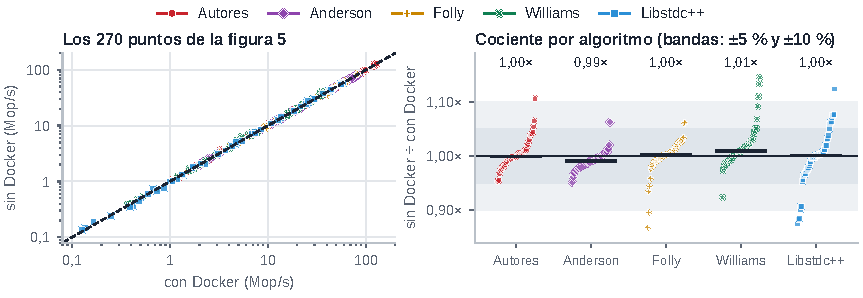
\includegraphics[width=\linewidth]{figuras/s48}
  \vfill\raggedright
  \caja{De los 270 puntos de la figura 5, \textbf{236 cambian menos de un 5\,\% y 259 menos de un 10\,\%}. La mediana del cociente va de 0,99\por{} a 1,01\por{} según el algoritmo.}
  \nota{s48}
\end{frame}

\begin{frame}{La figura 5 sin Docker: la misma historia}
  \fuente{nativo\_oficial/rendimiento.csv; mediana de 5 rondas de 2\,s}
  \centering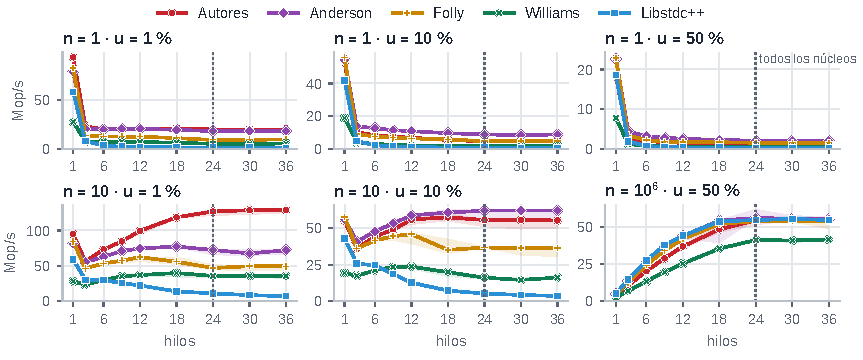
\includegraphics[width=\linewidth]{figuras/s49}
  \nota{s49}
\end{frame}

\begin{frame}{Por qué Docker no cambia nada, y un control que lo confirma}
  \fuente{controles.csv, control «docker»; EXPLICACION.md, Parte 6.6}
  \begin{columns}[T]
    \column{0.47\textwidth}
    \porque{un contenedor no es una máquina virtual}{Un contenedor es un proceso normal de Linux con otra vista del sistema de archivos y sus propios espacios de nombres. Usa el mismo núcleo, la misma CPU y la misma memoria. No hay un procesador simulado ni una capa que traduzca instrucciones: el código atómico se ejecuta igual.}
    \column{0.49\textwidth}
    \sub{Control: el mismo código dentro y fuera}\footnotesize
    Se compiló \texttt{bench.cpp} dentro y fuera del contenedor y se midió alternando un punto fuera y el mismo dentro, en orden al azar: 48 puntos, 3 rondas.
    \par\medskip\small
    \begin{tabular}{@{}lrrr@{}}
      \toprule
      \textbf{Dentro ÷ fuera} & \textbf{Mediana} & \textbf{Mín.} & \textbf{Máx.}\\
      \midrule
      48 puntos & \textbf{1,02\por} & 0,91\por & 1,13\por\\
      \bottomrule
    \end{tabular}
    \par\smallskip\scriptsize
    El máximo, +13\,\% con 1 hilo, tampoco es de Docker: dentro hay otro compilador, otra biblioteca C y otro jemalloc.
  \end{columns}
  \vfill
  \caja{\textbf{Conclusión:} las diferencias entre tandas vienen del \textbf{programa}, no del contenedor. No se puede descartar del todo que dos efectos contrarios se anulen, pero tendrían que hacerlo en los 270 puntos a la vez.}
  \nota{s50}
\end{frame}

\begin{frame}{Las dos excepciones, y por qué no se pueden achacar a Docker}
  \fuente{docker y nativo\_oficial: rendimiento.csv (pares) y latencia.csv; EXPLICACION.md, Parte 6.6}
  \begin{columns}[T]
    \column{0.47\textwidth}
    \sub{1. Williams con dos hilos en clústeres distintos}\small
    \begin{tabular}{@{}lr@{}}
      \toprule
      & \textbf{Mop/s}\\
      \midrule
      Con Docker & 0,09\\
      Sin Docker & 0,70\\
      Mismo clúster, en ambos & unos 3\\
      \bottomrule
    \end{tabular}
    \par\medskip\footnotesize
    Se hunde en los dos casos, pero mucho más dentro. Williams usa \texttt{boost::atomic}, y Boost cambia de 1.74 a 1.83. Es una sospecha: se ve en la \hyperlink{parte9}{parte 9}.
    \column{0.49\textwidth}
    \sub{2. La latencia con contención}\small
    \begin{tabular}{@{}lr@{}}
      \toprule
      \textbf{Williams, \texttt{load}, $p = 24$} & \textbf{Mediana}\\
      \midrule
      Con Docker, 5 rondas & 3\,104\,ns\\
      Sin Docker, 15 rondas & 6\,106\,ns\\
      \bottomrule
    \end{tabular}
    \par\medskip\footnotesize
    Parece mucho, pero la misma medida cambia todavía más de una ronda a otra: la ronda más lenta llega a ser 37 veces la más rápida. Esta diferencia no sirve para juzgar a Docker (\hyperlink{parte7}{parte 7}).
  \end{columns}
  \vfill
  \caja{Todo lo demás sale casi calcado sin Docker: memoria retenida, efecto de separar los hilos y latencia sin contención.}
  \nota{s51}
\end{frame}
